\documentclass[
  bibliography=totoc,     % Literatur im Inhaltsverzeichnis
  captions=tableheading,  % Tabellenüberschriften
  titlepage=firstiscover, % Titelseite ist Deckblatt
]{scrartcl}

% Paket float verbessern
\usepackage{scrhack}

% Warnung, falls nochmal kompiliert werden muss
\usepackage[aux]{rerunfilecheck}

% unverzichtbare Mathe-Befehle
\usepackage{amsmath}
% viele Mathe-Symbole
\usepackage{amssymb}
% Erweiterungen für amsmath
\usepackage{mathtools}

% Fonteinstellungen
\usepackage{fontspec}
% Latin Modern Fonts werden automatisch geladen
% Alternativ:
%\setromanfont{Libertinus Serif}
%\setsansfont{Libertinus Sans}
%\setmonofont{Libertinus Mono}
\recalctypearea % Wenn man andere Schriftarten gesetzt hat,
% sollte man das Seiten-Layout neu berechnen lassen

% deutsche Spracheinstellungen
\usepackage{polyglossia}
\setmainlanguage{german}


\usepackage[
  math-style=ISO,    % ┐
  bold-style=ISO,    % │
  sans-style=italic, % │ ISO-Standard folgen
  nabla=upright,     % │
  partial=upright,   % ┘
  warnings-off={           % ┐
    mathtools-colon,       % │ unnötige Warnungen ausschalten
    mathtools-overbracket, % │
},                       % ┘
]{unicode-math}

% traditionelle Fonts für Mathematik
\setmathfont{Latin Modern Math}
% Alternativ:
%\setmathfont{Libertinus Math}

\setmathfont{XITS Math}[range={scr, bfscr}]
\setmathfont{XITS Math}[range={cal, bfcal}, StylisticSet=1]

% Zahlen und Einheiten
\usepackage[
locale=DE,                   % deutsche Einstellungen
separate-uncertainty=true,   % immer Fehler mit \pm
per-mode=symbol-or-fraction, % / in inline math, fraction in display math
]{siunitx}

% chemische Formeln
\usepackage[
version=4,
math-greek=default, % ┐ mit unicode-math zusammenarbeiten
text-greek=default, % ┘
]{mhchem}

% richtige Anführungszeichen
\usepackage[autostyle]{csquotes}

% schöne Brüche im Text
\usepackage{xfrac}

% Standardplatzierung für Floats einstellen
\usepackage{float}
\floatplacement{figure}{htbp}
\floatplacement{table}{htbp}

% Floats innerhalb einer Section halten
\usepackage[
section, % Floats innerhalb der Section halten
below,   % unterhalb der Section aber auf der selben Seite ist ok
]{placeins}

% Seite drehen für breite Tabellen: landscape Umgebung
\usepackage{pdflscape}

% Captions schöner machen.
\usepackage[
  labelfont=bf,        % Tabelle x: Abbildung y: ist jetzt fett
  font=small,          % Schrift etwas kleiner als Dokument
  width=0.9\textwidth, % maximale Breite einer Caption schmaler
]{caption}
% subfigure, subtable, subref
\usepackage{subcaption}

% Grafiken können eingebunden werden
\usepackage{graphicx}
% größere Variation von Dateinamen möglich
\usepackage{grffile}

% schöne Tabellen
\usepackage{booktabs}

% Verbesserungen am Schriftbild
\usepackage{microtype}

% Literaturverzeichnis
\usepackage[style=alphabetic,]{biblatex}
% Quellendatenbank
\addbibresource{lit.bib}
\addbibresource{programme.bib}

% Hyperlinks im Dokument
\usepackage[
  unicode,        % Unicode in PDF-Attributen erlauben
  pdfusetitle,    % Titel, Autoren und Datum als PDF-Attribute
  pdfcreator={},  % ┐ PDF-Attribute säubern
  pdfproducer={}, % ┘
]{hyperref}
% erweiterte Bookmarks im PDF
\usepackage{bookmark}

% Trennung von Wörtern mit Strichen
\usepackage[shortcuts]{extdash}

\title{V606: Messung der Suszeptibilität paramagnetischer Substanzen}
\author{
  Simon Schulte
  \texorpdfstring{
    \\
    \href{mailto:simon.schulte@udo.edu}{simon.schulte@udo.edu}
  }{}
  \texorpdfstring{\and}{, }
  Tim Sedlaczek
  \texorpdfstring{
    \\
    \href{mailto:tim.sedlaczek@udo.edu}{tim.sedlaczek@udo.edu}
  }{}
}
\publishers{TU Dortmund – Fakultät Physik}

\date{Durchführung: 13.06.2017\\
      Abgabe: 20.06.2017}


\begin{document}

\maketitle
\thispagestyle{empty}
\tableofcontents
\newpage
\setcounter{page}{1}
\section{Zielsetzung}
\label{sec:zielsetzung}
Ziel des Versuchs ist es, die Suszeptibilität von Seltenen-Erd-Elementen zu bestimmen.
\section{Theorie}
\label{sec:theorie}
Es werden seltene Erden genutzt, da die Ionen von seltenen Erden stark
paramagnetisch sind. Das heißt, dass deren Drehimpuls nicht verschwindet.
Dabei ergibt sich der Gesamtdrehimpuls eines Atoms aus dem Bahndrehimpuls
der Elektronenhülle, dem Spin der Elektronen und dem Kerndrehimpuls. Das
Nicht-Verschwinden des Drehimpulses ist gewährleistet, da durch verschiedene
Orientierungen der magnetischen Momente zu einem äußeren anliegenden Feld
immer wieder ein neuer Drehimpuls erzeugt wird. Zuerst wird die Suszeptibilität
berechnet. Dabei wird zuerst die magnetische Flussdichte
\begin{equation}
  \vec{B}\,=\,\mu_0 \vec{H} + \vec{M}
  \label{eqn:B}
\end{equation}
betrachtet, durch welche dann die Magnetisierung selbst bestimmt wird:
\begin{equation}
  \vec{M}\,=\,\mu_0 \chi \vec{H}
  \label{eqn:M}
\end{equation}
Dabei ist $\mu_0$ die Induktionskonstante, $\vec{M}$ die Magnetisierung,
$\vec{B}$ die Flussdichte und $\vec{H}$ die Feldstärke. $\chi$ ist die
Suszeptibilität. Die Suszeptibilität ist nicht konstant, sondern hängt
im Allgemeinen von der Temperatur $T$ und $\vec{H}$ ab. Die Temperatur
ist insofern relevant, als dass Temperatur im Allgemeinen abhängig von
Materie und ihrer Wechselwirkung miteinander ist. Durch Temperaturschwankungen
verändern Atome somit ihre Orientierung.
Der Gesamtdrehimpuls $\vec{J}$ der Elektronenhülle ergibt sich zu
\begin{equation}
  \vec{J}\,=\,\vec{L}+\vec{S}.
  \label{eqn:gesamtdrehimpuls}
\end{equation}
Dabei bezeichnet $\vec{L}$ der Gesamtbahndrehimpuls und $\vec{S}$ den Gesamtspin.
Abbildung \ref{fig:V6061} zeigt das Vektordiagramm aus den Drehimpulsvekoren einer Elektronenhülle.
\begin{figure}[H]
  \centering
  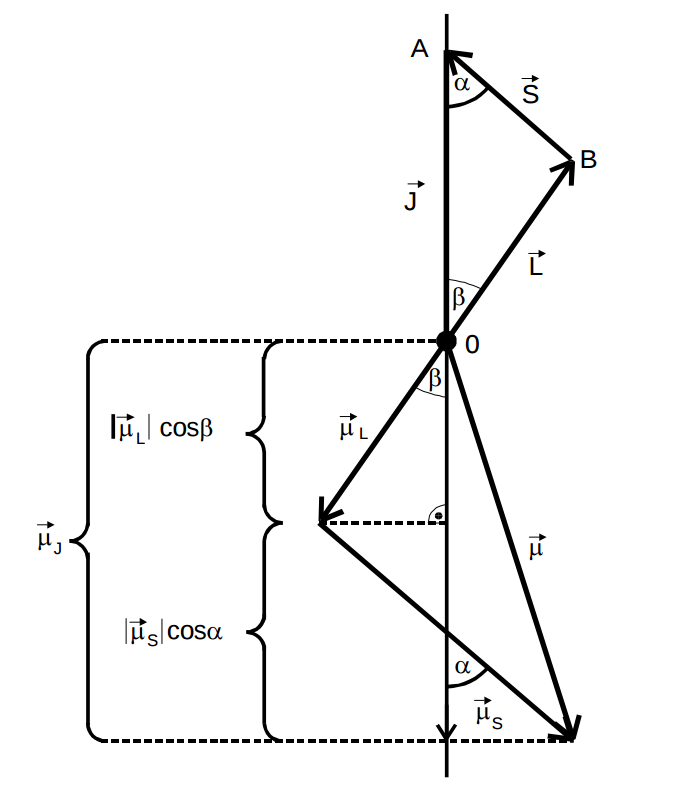
\includegraphics[width=0.7\textwidth]{V6063.png}
  \caption{Das Vektordiagramm aus den Drehimpulsvektoren einer Elektronenhülle
  und die daraus resultierenden magnetischen Momenten. \cite{anleitung}}
  \label{fig:V6061}
\end{figure}
\noindent
Aus geometrischen Gesetzen und einigen Umformungen erhält man damit den sogenannte Lande-Faktor
\begin{equation}
  g_J\,=\, \frac{3J(J+1)+ (S(S+1)-L(L+1))}{2J(J+1)}.
  \label{eqn:g_j}
\end{equation}
Durch Berücksichtigung der Richtungsquantelung, welche besagt, dass nur Winkel
zwischen der Richtung des äußeren Magnetfeldes und der Lage von $\vec{\mu}_J$
möglich sind, dessen Komponenten $\mu_{J_Z}$ und $\vec{\mu}_J$ in Feldrichtung
ein ganzzahliges Vielfaches von
\begin{equation}
  \mu_{J_Z} \,=\,- \mu_B g_J m
  \label{eqn:mu}
\end{equation}
ist und einigen mathematischen Umformungen ergibt sich für die Suszeptibilität
\begin{equation}
  \chi \,=\, \frac{\mu_0 \mu_B^2 g_J^2 NJ(J+1)}{3kT}.
  \label{eqn:xi}
\end{equation}
Dabei ist
\begin{equation*}
  \mu_B\,\coloneq\,\frac{1}{2} \frac{e_0}{m_0} \hbar
\end{equation*}
und $m$ die Orientierungsquantenzahl.
Das Curiesche Gesetz des Paramagnetismus, welches einen Zusammenhang zwischen
Temperatur und Suszeptibilität liefert, ergibt sich dabei zu
\begin{equation}
  \chi\,\approx\,\frac{1}{T}.
\end{equation}
Die Suszeptibilität lässt sich auch durch mathematische Umformungen und einige
Abschätzungen auch als
\begin{equation}
  \chi\,=\,2\frac{\symup{\Delta}R}{R_3} \frac{F}{Q}
  \label{eqn:xi2}
\end{equation}
beschreiben. Dabei ergibt sich für
\begin{equation*}
  \symup{\Delta}R\,=\,\chi \frac{R_3}{2} \frac{Q}{F}.
\end{equation*}
Außerdem ist $F$ der Querschnitt der Spule und $Q$ der Querschnitt der Probe.
Wenn nun $\omega -> \infty$ betrachtet wird  ergibt sich für die Suszeptibilität
\begin{equation}
  \chi\,=\,4 \frac{F}{Q} \frac{U_{Br}}{U_{Sp}}.
  \label{eqn:infty}
\end{equation}
Die Seltenen-Erd-Elemente haben die Besonderheit, dass ihre Ionen paramagnetisch sind. Damit lässt sich bei Seltenen-Erd-Elementen gut die Suszeptibilität berechnen. Suszeptibilität ist abhängig von der Anordnung von Elektronen im Atom. Aus den Elektronen resultiert der Gesamtdrehimpuls. Dabei gibt es drei Regeln, die durch die Hund'schen Regeln beschrieben werden.
Die Hund'schen Regeln sagen aus, dass die Spins sich zum maximalen Gesamtspin kombinieren. Dies ist auf das Pauli-Prinzip zurückzuführen, welches besagt, dass jedes Elektron sich in einer Atomhülle in mindestens einer seiner Quantenzahlen von seinem Nachbarn unterscheiden muss. Damit können sich auf einer Schale nie unendlich viele Elektronen aufhalten. Eine weitere Regel ist, dass sich der maximale Drehimpuls aus einzelnen Bahndrehimpulsen zusammensetzt, die mit der Pauli-Regel verträglich sind. Die letzte Regel besagt, dass der Gesamtdrehimpuls eine besondere Abhängigkeit vom maximalen Gesamtspin und vom maximalen Drehimpuls hat. Wenn die jeweilige Schale weniger als halb gefüllt ist ergibt sich der Zusammenhang
\begin{equation*}
  \vec{J}\,=\,\vec{L}-\vec{S}
  \label{eqn:-}
\end{equation*}
und wenn die Schale mehr als halb gefüllt ist ergibt sich der Zusammenhang
\begin{equation}
  \vec{J}\,=\,\vec{L}+\vec{S}.
  \label{eqn:+}
\end{equation}
\section{Versuchsaufbau}
\label{sec:aufbau}
Abbildung \ref{fig:V6062} zeigt den verwendeten Versuchsaufbau zur Bestimmung
der Suszeptibilität. Ein Sinusgenerator führt eine Speisespannung in eine
Brückenschaltung ein. Die Brückenschaltung hat ein Fach für die
Seltene-Erd-Elemente. Das Signal und die Veränderung des Signals
werden von verschiedenen Verstärkern verstärkt und an dem AC-Milli-voltmeter
werden dann die Spannungen abgelesen.
\begin{figure}[H]
  \centering
  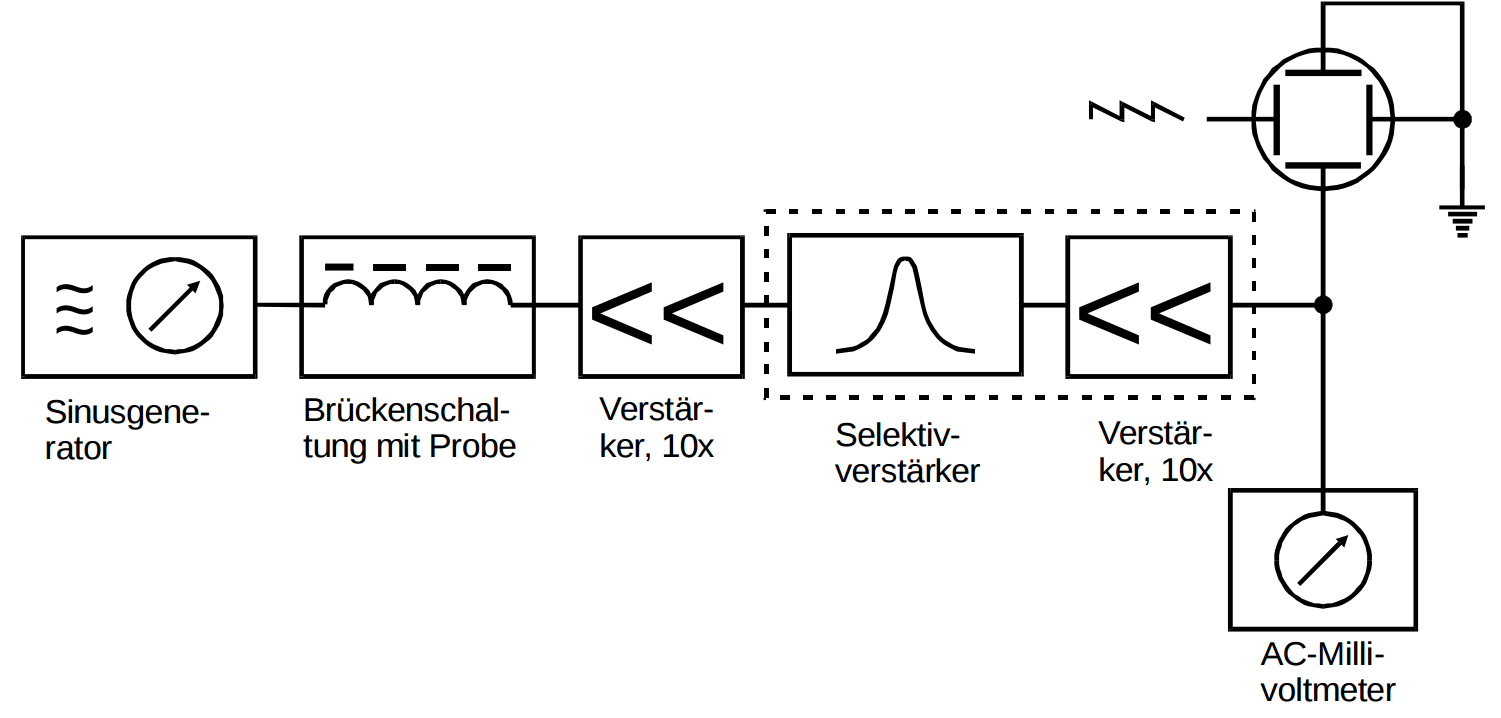
\includegraphics[width=0.9\textwidth]{V6062.png}
  \caption{Das Blockschaltbild der verwendeten Messapparatur. \cite{anleitung}}
  \label{fig:V6062}
\end{figure}
\noindent

\begin{figure}[H]
  \centering
  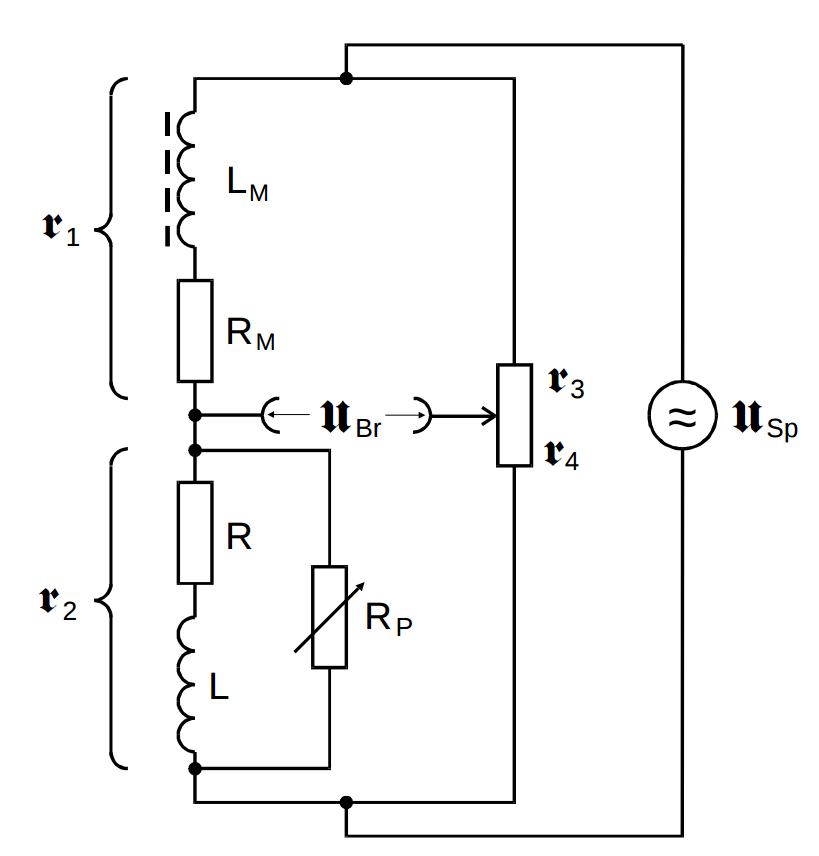
\includegraphics[width=0.7\textwidth]{V6061.png}
  \caption{Die Brückenschaltung für die Suszeptibilitätsmessung \cite{anleitung}}
  \label{fig:V6063}
\end{figure}
\noindent
Abbildung \ref{fig:V6063} zeigt die verwendete Brückenschaltung. Dabei geht
eine Speisespannung, die nicht über $\SI{1}{\volt}$ liegen sollte, in die
Brückenschaltung ein. Dort trifft sie auf Widerstände und Spulen. Es werden
zwei Spulen gleicher Induktivität genutzt. Ebenso sind die beiden Widerstände
$R$ und $R_M$ gleich.
\section{Versuchsdurchführung}
\label{sec:durchführung}
Zunächst wird die Ausgangsspannung $U_A$ vom Selektivverstärker in Abhängigkeit
von der Frequenz bestimmt, um eine Durchlasskurve zu erhalten. Dabei ist die
Eingangsspannung $U_E$ konstant. Das Signal stammt von einem Synthesizer und
es wird am Selektivverstärker eingestellt, dass dieser eine Durchlassfrequenz
zwischen \SI{30000}{\hertz} und \SI{40000}{\hertz} hat. Dann wird die
Filterkurve dieses Selektivverstärkers bei einer Güte von $Q=100$ aufgenommen.
Es werden 33 Werte in einem Abstand von $\SI{300}{\hertz}$ aufgenommen.
Als nächstes wird die Suszeptibilität der Oxiden von einigen
Seltener-Erd-Elementen bestimmt. Dazu wird der Aufbau, der in Abbildung
\ref{fig:V6063} zu sehen ist, genutzt. Dabei wird zuerst die Brücke ohne
Probe nach Null abgeglichen. Dazu werden die Abgleichelemente der Brücke
verändert. Dann wird die Brückenspannung $U_{Br}$ bestimmt. Danach wird
erneut nach Null abgeglichen. Dabei ergeben sich verschiedene Widerstände
und aus der Differenz dieser erlangt man die Suszeptibilität der Elemente.
Es werden jeweils 3 Messungen für 3 verschiedene Speisespannungen für 3
verschiedene Seltene-Erd-Elemente durchgeführt.
\noindent
Dabei werden drei Proben mit den folgenden Massen und Längen genutzt. \\
\\
Für die $Nd_2O_3$-Probe ergibt sich
\begin{align*}
  m\,&=\,\SI{9}{\gram} \\
  l\,&=\,\SI{16.5}{\centi\meter}
\end{align*}
Für die $Gd_2O_3$-Probe ergibt sich
\begin{align*}
  m\,&=\,\SI{14.08}{\gram} \\
  l\,&=\,\SI{16.7}{\centi\meter}
\end{align*}
Für die $Dy_2O_3$-Probe ergibt sich
\begin{align*}
  m\,&=\,\SI{15.1}{\gram} \\
  l\,&=\,\SI{15.8}{\centi\meter}
\end{align*}
\section{Fehlerrechnung}
\label{sec:fehlerrechnung}
Die in der Auswertung verwendeten Mittelwerte mehrfach gemessener Größen sind
gemäß der Gleichung
\begin{equation}
    \bar{x}=\frac{1}{n}\sum_{i=1}^n x_i
    \label{eqn:mittelwert}
\end{equation}
bestimmt. Die Standardabweichung des Mittelwertes ergibt sich dabei zu
\begin{equation}
    \mathup{\Delta}\bar{x}=\sqrt{\frac{1}{n(n-1)}\sum_{i=1}^n\left(x_i-\bar{x}\right)^2}.
    \label{eqn:standardabweichung}
\end{equation}
Resultiert eine Größe über eine Gleichung aus zwei oder mehr anderen
fehlerbehafteten Größen, so berechnet sich der Gesamtfehler nach der
Gaußschen Fehlerfortpflanzung zu
\begin{equation}
    \mathup{\Delta}f(x_1,x_2,...,x_n)=\sqrt{\left(\frac{\partial f}{\partial x_1}\mathup{\Delta}x_1\right)^2+\left(\frac{\partial f}{\partial x_2}\mathup{\Delta}x_2\right)^2+ \dotsb +\left(\frac{\partial f}{\partial x_n}\mathup{\Delta}x_n\right)^2}.
    \label{eqn:fehlerfortpflanzung}
\end{equation}
Alle in der Auswertung angegebenen Größen sind stets auf die erste signifikante
Stelle des Fehlers gerundet. Setzt sich eine Größe über mehrere Schritte aus
anderen Größen zusammen, so wird erst am Ende gerundet, um Fehler zu vermeiden.
Zur Auswertung wird das Programm Python verwendet.
\clearpage
\section{Auswertung}
\label{sec:auswertung}

\end{document}
